\chapter{Analýza}\label{analuxfdza}

Jak je zvykem u~organizovaného vývoje softwaru --- implementaci a~návrhu
aplikace předchází analýza, pro stanovení požadavků uživatelů softwaru a
upřesnění funkcionalit aplikace.

Následující kapitola se takovou analýzou zabývá. Jsou zde analyzována
existující řešení, zjištěno, co požadují návštěvníci herny a
zaměstnanci pracující v~herně, a~jaké požadavky jsou realizovatelné.

\section{Analýza existujících řešení
výuky}\label{analuxfdza-existujuxedcuxedch-ux159eux161enuxed-vuxfduky}

Výukové aplikace pro seznámení s~virtuální realitou již existují,
nicméně, většina z~nich trpí špatnou přístupností. Jsou navrhovány tak,
že po absolvování výukového bloku již nejsou jednoduše dostupné. Jsou tak
obtížně spustitelné opakovaně.

Takové aplikace jsou spíše určené pro toho, kdo jako první systém
konfiguruje a~je jeho prvním uživatelem. Nově příchozím
k~již nakonfigurovanému systému není tutoriál nabídnut a~je přímo uveden do
prostředí, ve kterém se očekává, že uživatel již systém důvěrně zná.

\newpage 

Součásti následující analýzy je i porovnání jednotlivých existujících řešení, pro
které jsou stanoveny následující metriky k~porovnání:

\begin{itemize}
\tightlist
\item
  jednoduchost přístupu k~výukové aplikaci
\item
  rychlost a~svižnost výuky
\item
  zábavnost
\item
  výstižnost
\item
  srozumitelnost
\end{itemize}

\subsection{SteamVR Tutorial}\label{steamvr-tutorial}

Pro totožnou platformu, pro kterou je aplikace této práce
určena existuje oficiální výuková aplikace vytvořená přímo společností
\emph{Valve}.

\subsubsection{Průběh výuky}\label{prux16fbux11bh-vuxfduky}

Aplikace se nejprve uvede vizuálně poutavým úvodem, který spočívá
v~sestavení výukové scény animací obklopující uživatele. Uživateli je tak nenuceně
ukázána možnost rozhlížet se kolem sebe a~prozkoumávat prostředí, což
většina uživatelů intuitivně udělá.

Následně je uživateli představena postava \emph{Virtual Reality
Assistance and Education Core} z~prostředí hry Portal 2, která s~uživatelem
komunikuje a~provádí ho výukou --- stává se tak \emph{průvodcem}. Monolog
je dabovaný a~v~místech, kde se nachází průvodce se zobrazují titulky,
které jsou lokalizovány do nepřeberného množství jazyků (i češtiny).

Příjemným bonusem je pro hráče hry Portal 2 familiarita postavy, která
může zvýšit pozornost, a~pro hráče, kteří si hru Portal 2
v~minulosti oblíbili, tak tutoriál navozuje na obličejích úsměv.

\begin{figure}[h!]
\centering
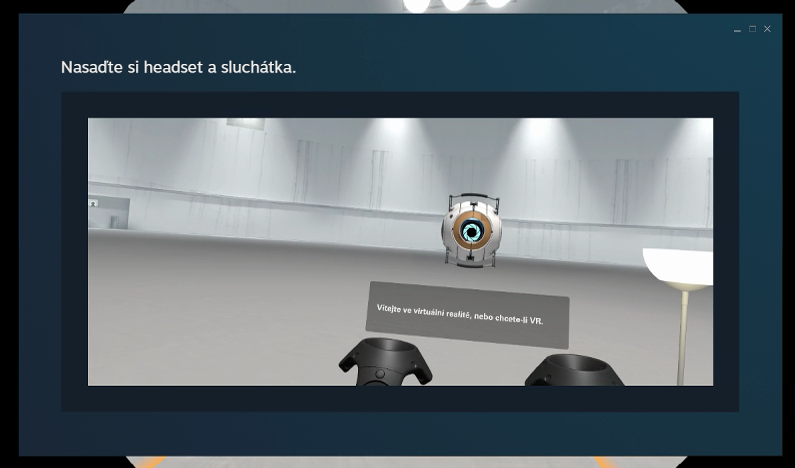
\includegraphics[width=12cm]{src/assets/steamvr-tutorial.png}
\caption{Výuková aplikace SteamVR Tutorial}
\end{figure}

Jako první je uživateli představena plocha, tzv. \emph{play area}, ve
které se VR~zážitky budou odehrávat. Neprodleně jsou pak představeny
tzv. \emph{chaperone bounds}, které upozorňují na skutečnost opouštění 
hranice \emph{play area}. Protože je tato funkcionalita
důležitá pro uživatelovu bezpečnost, je na ni ve výuce kladen důraz a~je proto
požádán, aby se ke kraji místnosti pomalu přiblížil a~následně to stejné
zopakoval na druhé straně místnosti.

Dále je uživatel požádán, aby se podíval na ovladače, které drží v~ruce
a~provedl s~nimi libovolné pohyby pro vyzkoušení manipulace.
Poté, co se seznámí s~ovladačem, jsou mu postupně představena
všechna tlačítka, která se nachází na ovladači. Je požádán, aby každé
stiskl a~vyzkoušel si, kde se nacházejí a~jakou mají zpětnou odezvu.

Výuková aplikace je pojatá spíše komicky a~každé tlačítko velmi chytře
vyvolává různé destrukční, hlasité a~nečekané události, které se
průvodci příliš nelíbí. Průvodce uživatele po chvíli žádá, aby s~opakovaným
mačkáním přestal. Uživatel však může mít zlé úmysly a~nutkání tyto tlačítka
stisknout opakovaně, aby průvodce rozčílil a~dělal nepořádek. Tím se
však s~tlačítky seznámí o~to více.

Uživatel není informován o~tom, která tlačítka mají jakou funkci, logicky
z~důvodu, že každá VR~aplikace má své vlastní pojetí smyslu těchto
tlačítek. Pouze k~tlačítkům \emph{Menu} a \emph{System} je uživateli
řečeno, k~čemu se nejčastěji používají.

Uživatel je požádán o~stisk tlačítka \emph{System}, což vede k~otevření
\emph{SteamVR Dashboard}. Lze si povšimnout, že se výuka při oteření
nepozastaví, a~probíhá tak stále instruktáž, jak se lze ve \emph{SteamVR
Dashboard} pohybovat a~k~čemu je určena.

Tím výuka končí. Uživatel je instruován k~otevření
\emph{Dashboardu} (pokud jej opustil) a~výběrem VR~aplikace. Může však
v~aplikaci zůstat a~dále zkoušet práci s~ovladači, nebo zhlédnout
závěrečnou animaci, kdy průvodce komicky odvezou jiné postavy pryč ze
scény.

\subsubsection{Zhodnocení}\label{zhodnocenuxed}

SteamVR Tutorial je dobrým příkladem výukové aplikace. Je kvalitně
navržena, spíše se strohým, ale kvalitním vizuálním a~zvukovým
zpracováním.

Pro účely herny je však shledána za nevhodnou, jelikož je návštěvníkům herny
taková aplikace prakticky nepřístupná. Obsluha je nucena ji spustit
manuálně a~také se návštěvníka herny zeptat, jestli už výuku absolvoval
a~zda ji chce skutečně absolvovat. Návštěvník nemá možnost si takovou
výuku spustit sám, zopakovat ji, nebo alespoň po absolvování získat
nějaký závěrečný přehled, pro zopakování toho, co se naučil.

\begin{figure}[h!]
\centering
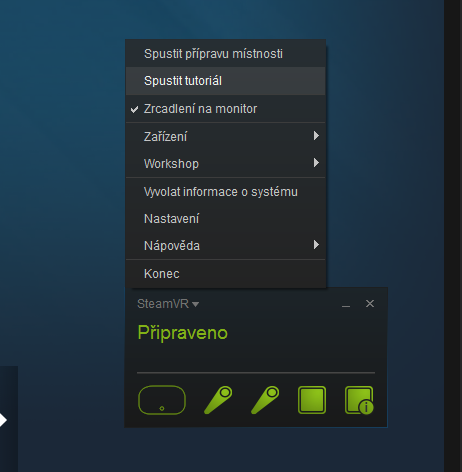
\includegraphics[height=8cm]{src/assets/hidden-menu.png}
\caption{Přístup k~aplikaci je skryt ve SteamVR nabídce, která je
přístupna jen z~monitoru počítače}
\end{figure}

Další nevýhodou je délka tutoriálu, která se běžně pohybuje kolem 6--11
minut. To představuje v~prostředí, kde se běžně systém zapůjčuje na
jednu hodinu, velkou část vyhrazeného času.

\subsection{Oculus Touch Tutorial \& Oculus First
Contact}\label{oculus-touch-tutorial-oculus-first-contact}

Pro konkurenční systém \emph{Oculus Rift} a~jeho platformu je určena
aplikace \emph{Oculus First Contact}, která je spojena s~předcházející
krátkou výukou k~ovladačům \emph{Oculus Touch}, které jsou k~systému
\emph{Oculus Rift} prodávány odděleně. Bez těchto ovladačů tuto výuku
nelze absolvovat.

\subsubsection{Průběh výuky}\label{prux16fbux11bh-vuxfduky-1}

Uživatel je zasazen do čistého prostředí, bez předmětů, zobrazující
pouze ovladače v~ruce. Před ním se pak zobrazuje přepis (titulky) hlasu
průvodkyně, která není vizuálně zpracována, lze slyšet pouze hlas.

Jako první je požádán, aby se podíval na podlahu a~zpozoroval obrys
prostoru, ve kterém se může uživatel pohybovat (\emph{play area}).
Následně je požádán, aby se podíval na své ruce a~ovladače, které drží,
a~osahal si všechna tlačítka, která se mu podaří nalézt. Následně jsou
mu všechna tlačítka jedno po druhém představeny. Jsou postupně
zvýrazněny a~je požádán, aby tato tlačítka stiskl.

\begin{figure}[h!]
\centering
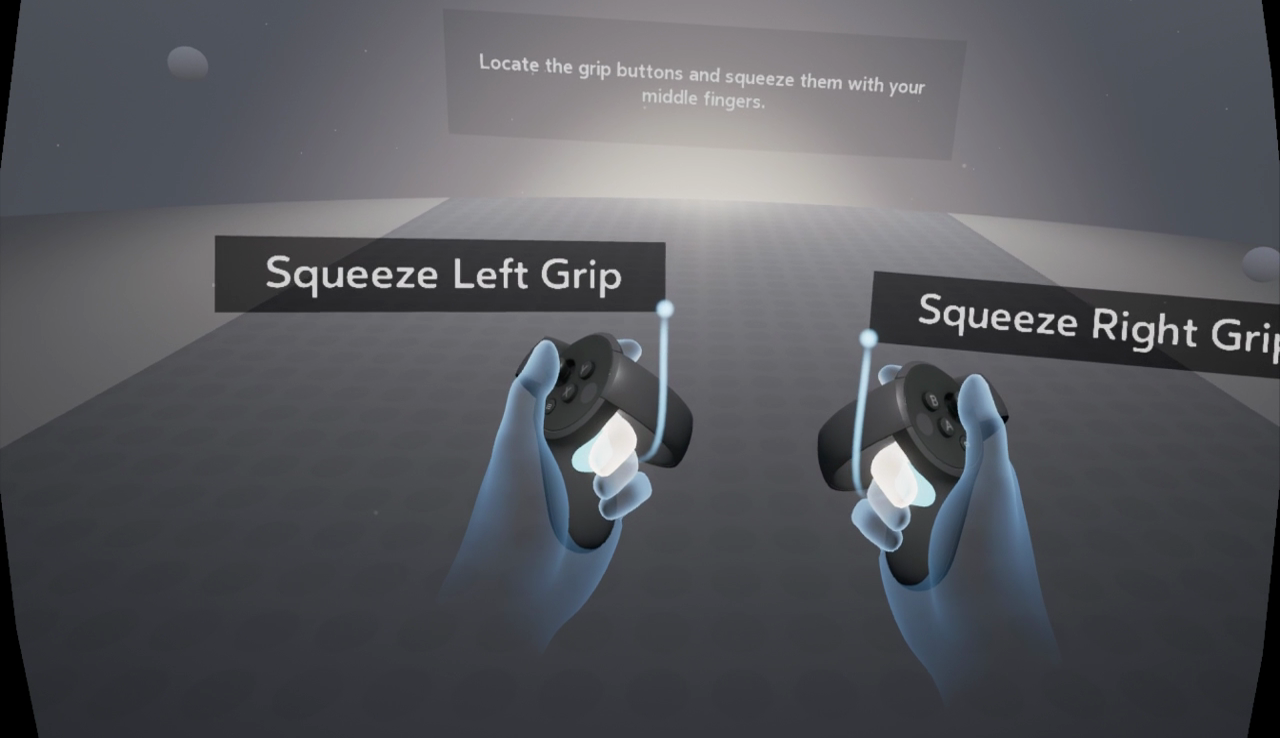
\includegraphics[width=12cm]{src/assets/oculus-tutorial.png}
\caption{Výuková aplikace Oculus Touch Tutorial}
\end{figure}

Pokud uživatel provádí stisky tlačítek svižně, lze tuto část projít
rychleji. Výuka nezdržuje dlouhým monologem nebo pauzami. Jde o~krátké
věty a~díky tomu působí velmi svižně.

Vzápětí jsou uživateli ovladače vizuálně z~rukou odstraněny a~je
požádán, aby znovu vyzkoušel stisknout tlačítka a~zvedat z~nich prsty
tak, aby pochopil reprezentaci přirozeného pohybu rukou a~prstů, kterou
se ovladače \emph{Oculus Touch} od konkurence liší. 

Je požádán, aby
stiskl specifické kombinace tlačítek takovým způsobem, aby vytvářel
gesta rukou, jako je například gesto uzavření v~pěst nebo míření na
objekty ukazováčkem.

Uživateli není vysvětlen účel tlačítek, z~dříve zmíněných důvodů. Pokud
však předpokládáme, že všechny VR~aplikace a~hry budou implementovat
systém gest ruky, které byly vysvětleny v~třetí části výuky, uživatel je
schopen odvodit účel tlačítek sám, což lze považovat za nespornou
výhodu.

Překvapující je absence objasnění smyslu tlačítek \emph{Oculus} a
\emph{Menu}, které většinou ve všech VR~aplikacích mají totožný účel.

Tím výuka končí a~je spuštěna aplikace \emph{Oculus First Contact},
která je určena k~prohloubení právě nabytých znalostí a~slouží jako
úvodní zábavný zážitek, který je srovnatelně kvalitní a~zábavný, jako
jiné herní tituly pro virtuální realitu. Tímto krokem lze považovat výuku
za dokončenou a~aplikací \emph{Oculus First Contact} začíná
,,zábava''.

\begin{figure}[h!]
\centering
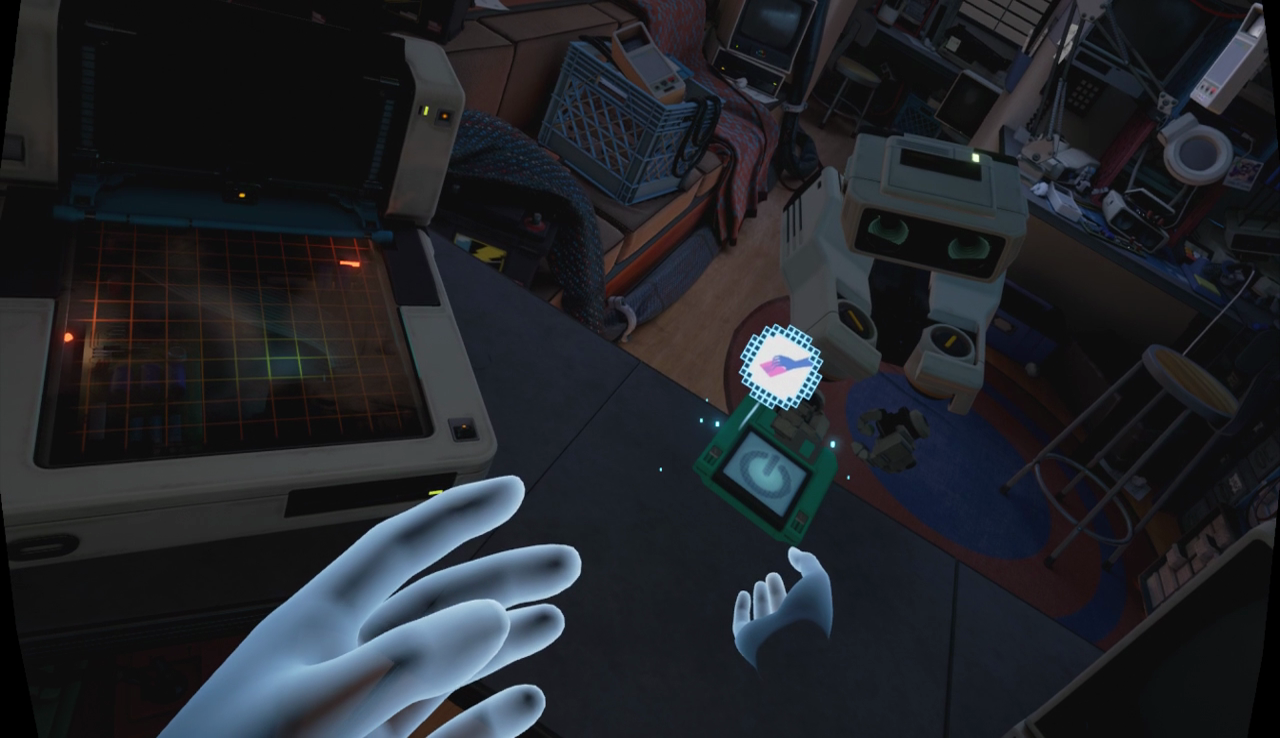
\includegraphics[width=12cm]{src/assets/oculus-first-contact.png}
\caption{Aplikace Oculus First Contact}
\end{figure}

\subsubsection{Zhodnocení}\label{zhodnocenuxed-1}

\emph{Oculus} má výukovou aplikaci zpracovanou do podstatně rychlejšího
tempa, než \emph{SteamVR}. Přispívá tomu i oddělení ryze výukové části od zábavy. Nejprve přichází rychlý a~strohý úvod ovládání, který trvá
přibližně 4--5 minut. Až po tomto úvodu následuje zábavný prvek
ve formě plnohodnotného VR~zážitku. Vidíme tak zásadní rozdíl oproti
SteamVR, který tyto dva prvky míchá do spojeného průběhu.

\section{Analýza existujících řešení
spouštěčů}\label{analuxfdza-existujuxedcuxedch-ux159eux161enuxed-spouux161tux11bux10dux16f}

Po skončení výuky můžeme předpokládat, že návštěvník herny je se
systémem do určité míry seznámen, nicméně, následně je mu nutné nějakým způsobem
nabídnout výběr VR~zážitků. Hernu může navštívit za obecným účelem vyzkoušet si virtuální realitu, nebo může mít předem vybranou aplikaci, kterou si do herny přichází vyzkoušet. První
zmíněný důvod je v~hernách vídán mnohem častěji.

Obě dříve zmíněné platformy (SteamVR a~Oculus) mají
vlastní software pro spouštění VR~aplikací. Ty jsou v~této kapitole
analyzovány.

\subsection{SteamVR Dashboard}\label{steamvr-dashboard}

\emph{SteamVR Dashboard} je pouze malou modifikací již existujícího
\emph{Steam Big Picture} --- rozhraní pro práci s~platformou
\emph{Steam}, přizpůsobené pro ovládání herním ovladačem.

U~hráčů počítačových her je velká pravděpodobnost, že se s~platformou
\emph{Steam} již v~minulosti setkali. Mnozí z~nich se také setkali i
s~rozhraním \emph{Big Picture}, někteří z~nich jej dokonce používají jako
primární rozhraní pro práci s~platformou \emph{Steam}. To představuje nespornou výhodu, protože takoví hráči se budou pohybovat ve
známém prostředí.

Na druhou stranu lze však považovat jako nevýhodu fakt, že \emph{Steam
Big Picture} nebyl původně navržen pro použití s~VR. Uživatel tak pracuje
s~malým oknem na virtualizovaném monitoru. Vidí před sebou plochu, na
kterou je rozhraní plošně promítáno. Není tak plně využito potenciálu VR
prostoru.

\begin{figure}[h!]
\centering
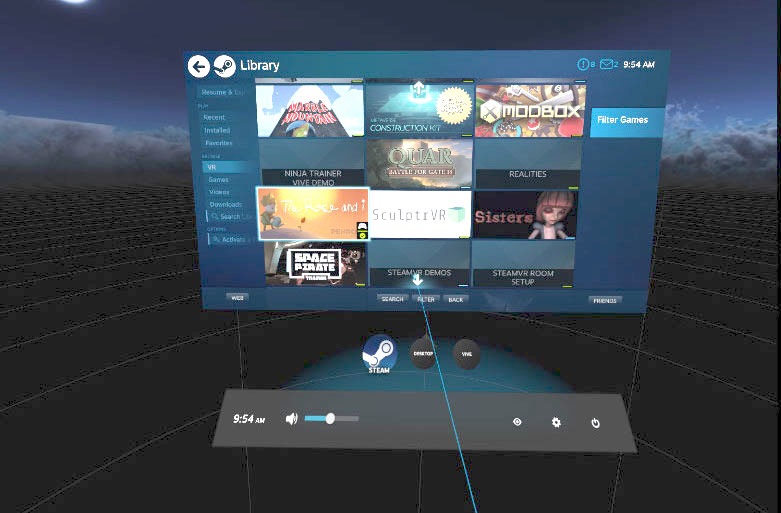
\includegraphics[width=12cm]{src/assets/steamvr-library.jpg}
\caption{SteamVR Dashboard \autocite{tomshardw}}
\end{figure}

Z~tohoto rozhraní lze procházet knihovnu her, prohlížet elektronický
obchod s~hrami, nakupovat v~něm, prohlížet komunitní profily, stránky
her, sledovat průběh aktuálního stahování, používat webový prohlížeč,
zobrazit monitor počítače, ovládat počítač a~přistupovat k~nastavení.

Pokud budeme hodnotit \emph{SteamVR Dashboard} z~pohledu návštěvníka
herny, je takové rozhraní nevyhovující. Pro návštěvníka, který nemá
s~platformou \emph{Steam} zkušenosti je rozhraní spíše matoucí a~může
vyžadovat určitou dobu, než se s~ním seznámí. 

V~rozhraní se nacházejí
sociální a~komunitní funkce, které pro použití v~herně nemají žádný
význam a~jsou jen dalším matoucím prvkem pro návštěvníka. Navíc je poskytnut
plný přístup k~obchodu a~kdokoliv by mohl na účet herny libovolně
nakupovat hry.

Seznam a~výběr VR~aplikací je pro použití v~herně taktéž spíše nevhodný.
Seznam se skládá z~mřížky 3x4 grafických bannerů, které o~dané hře, či aplikaci 
vypovídají jen málo. Je totiž na vývojářích, zda takovém banneru
zobrazí pouze logo, obrázek z~aplikace, či obojí. Lze tak velmi obtížně
odhadnout o~jaký žánr hry či typ aplikace jde, zda je zábavná, vizuálně přitažlivá, jaké
ovládání podporuje či zda může způsobit závratě a~kinetózu.

\subsection{Oculus Home}\label{oculus-home}

\emph{Oculus Home} je plnohodnotným rozhraním pro virtuální realitu od
společnosti Oculus pro svou stejnojmennou platformu. Narozdíl od
\emph{SteamVR Dashboard} je navržen přímo pro VR.

Skrze toto rozhraní lze procházet knihovnu her a~aplikací, či nakupovat hry
v~obchodě. Uživatel může vidět i minimální komunitní funkce, jakými jsou
seznam hráčů a~notifikace (a~to i systémové).

Rozhraní je vizuálně velmi přitažlivé. Zobrazuje se jako výchozí prostor
při nasazení headsetu na hlavu bez spuštěné aplikace, což oproti platformě
SteamVR, kde se zobrazuje prázdná šedá místnost s~mřížkou, působí lepším
dojmem.

\begin{figure}[h!]
\centering
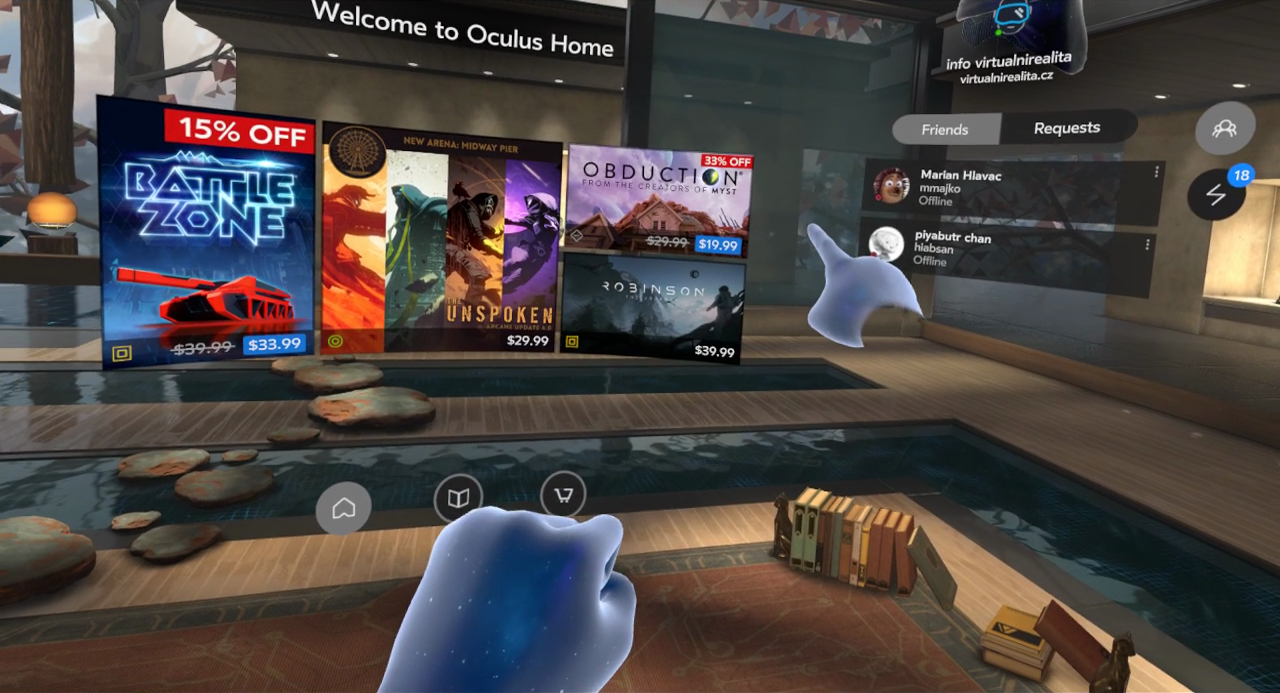
\includegraphics[width=12cm]{src/assets/oculus-home.png}
\caption{Oculus Home}
\end{figure}

Jelikož je rozhraní navržené specificky pro použití s~aplikacemi pro
virtuální realitu, k~hrám lze nalézt informace o~tom, jaké ovladače
podporuje a~lze je řadit podle míry ,,komfortu''. Nekomfortní hry a~aplikace jsou
pak označeny jako takové, které mohou způsobovat kinetózu. Díky tomu se
lidé, kterým se z~intenzivnějších zážitků dělá nevolno, mohou snadno podobným
hrám či aplikacím vyhnout.

V~prostředí herny je však \emph{Oculus Home} také mírně nevyhovující.
Přístup k~obchodu a~komunitní funkce jsou irelevantní účelu herny a
zbytečně odvádějí pozornost.

\section{Pozorování v~herně}\label{pozorovuxe1nuxed-v-hernux11b}

Ke konci března roku 2017 se naskytla příležitost stát se na jeden den
obsluhou v~herně \emph{Virtualnirealita.cz} v~pražských Dejvicích. Tato
příležitost byla využita v~prospěch analýzy, jako předmět pozorování a
bližšího pochopení požadavků zákazníků a~obsluhy herny.

Obsluha má povinnost seznámit zákazníky s~pronajatým
systémem. Pokud s~virtuální realitou neměli dosud zkušenost, nebo se
nedoslechli o~žádné konkrétní VR~aplikaci, kterou by si přišli
vyzkoušet, je nutné jim doporučit nějakou VR~aplikaci na základě jejich preferencí.

Aby bylo možné se zákazníky lépe pracovat a~doporučit jim správnou
aplikaci, sloužila k~tomuto účelu sada několika otázek. Z~odpovědí na ně vznikla
miniaturní analýza z~malého vzorku lidí, kteří ten den hernu navštívili.

Dotazování zákazníků se tak běžně skládalo z~otázek: 

\begin{itemize}
\tightlist
\item
,,Už jste u~nás
někdy byli?''
\item
  ,,Máte zkušenosti s~VR?''
\item
  ,,Hrajete počítačové hry?''
\item
  ,,Jaký žánr her rádi hrajete?''
\end{itemize}

Za daný den navštívilo hernu \textbf{15~zákazníků}, z~toho \textbf{10~mužů}. 
Většina --- \textbf{12~zákazníků} hraje počítačové hry, ale pouze
\textbf{2~z~nich} v~minulosti hernu navštívili, nebo měli s~VR
zkušenost. Většina z~nich byla mládež (v~rozmezí 15-30 let), výjimku
tvořili \textbf{2~děti} (\textless{}~15) a \textbf{2~dospělí}
(\textgreater{}~30). U~jednoho ze zákazníků se projevila
\emph{kinetóza}.

Pouze \textbf{4 z~nich} odpověděli, že jim nepřišly ovladače systému HTC
Vive obtížné na seznámení, stejně tak tito lidé odpověděli, že by se
obešli bez pomoci obsluhy. Dva z~těchto čtyř byli ti, kteří již s~VR
měli zkušenost.

Občasným jevem bylo několikanásobné vystřídání zákazníků na jednom
systému za dobu zapůjčení. To je důležitá informace, protože výuková
aplikace musí s~takovým jevem počítat. Rychlost seznámení se systémem
byla převážně ovlivněna zákazníkovou zkušenosti s~počítačovými hrami.

\section{Funkční požadavky zákazníků
herny}\label{funkux10dnuxed-poux17eadavky-zakazniku-herny}

Z~pozorování v~herně a~analýzy existujících řešení plynou následující
požadavky zákazníků herny.

\subsubsection*{F-A01 Uživatel se chce seznámit se základními pravidly systému
virtuální reality}
Uživatel chce vědět, jak se používá headset systému virtuální reality,
jak se může v~\emph{play area} pohybovat, kam se nesmí vydat a~jak je na
to upozorněn. Funkční požadavek je klíčový z~hlediska bezpečí
návštěvníka herny a~ochrany majetku herny.

\subsubsection*{F-A02 Uživatel se chce seznámit s~ovladači a~jejich tlačítky}
Uživatel chce vědět, jak vypadají ovladače, jakými tlačítky disponují a
k~čemu slouží. Tato znalost následně umožňuje uživateli pochopit ovládání v~konkrétních VR~aplikacích.

\subsubsection*{F-A03 Uživatel se chce seznámit s~funkcemi na tlačítkách pro
konkrétní hru}
Uživatel chce vědět, jak se ovládá konkrétní VR~aplikace.

\subsubsection*{F-A04 Uživatel si chce vybrat VR~aplikaci podle žánru}
Uživatel si chce zvolit VR~zážitek takového žánru, který mu vyhovuje. Do
herny docházejí různé věkové a~zájmové skupiny. Často záleží i na
pohlaví. Ženy většinou rády hrají méně intenzivnější zážitky, vyhýbají
se hororovým hrám a ,,střílečkám'' a~více ocení vizuálně atraktivní
aplikace. \autocite{ladiespreferences}

\subsubsection*{F-A05 Uživatel si chce vybrat VR~aplikaci podle intenzity}
Uživatel, u~kterého se projevuje kinetóza, si chce vybrat takovou
aplikaci, aby nebyla příliš intenzivní a~jeho zážitek z~VR~byl
pozitivní. Ač může být toto kritérium velmi subjektivní, lze aplikace
rozdělit alespoň do dvou kategorií, jako intenzivní a~klidné, kde pod
klidné aplikace spadají všechny aplikace, které mají implementovány
mechanismy zabraňující kinetóze, nebo nezahrnují pohyb kamery kinetózu
způsobující.

\subsubsection*{F-A06 Uživatel si chce vybrat VR~aplikaci podle vizuálního
zpracování}
Uživatel si chce vybrat takovou aplikaci, která bude pro něj vizuálně
atraktivní. Spousta uživatelů upřednostňuje určité aplikace
z~jednoduchého důvodu --- líbí se jim.

\subsubsection*{F-A07 Uživatel chce výuku kdykoliv přeskočit, nebo informace
zopakovat znova} 
Pokud uživatel shledá výuku subjektivně příliš
jednoduchou, či zdlouhavou, měl by mít možnost její průběh minimálně
urychlit. Naopak, pokud je pro něj výuka příliš rychlá, měl by mít na
konci výuky možnost si informace zopakovat, či zopakovat celou výuku
znova.

\subsubsection*{F-A08 Uživatel chce, aby byla výuka časově efektivní}
Protože má zákazník herny omezený čas, po který je mu zapůjčen systém
virtuální reality, je pro něj důležité, aby ho výuka o~tento čas
připravila v~co nejmenší míře.

\newpage

\section{Funkční požadavky obsluhy
herny}\label{funkux10dnuxed-poux17eadavky-obsluhy-herny}

Požadavky obsluhy se velkou částí kryje s~požadavky zákazníka, jen
z~jiného úhlu pohledu.

\subsubsection*{F-B01 Obsluha chce zákazníka seznámit s~pravidly používání
systému virtuální reality}
Aby uživatel používal systém správně, obsluha se potřebuje ujistit, že
zákazník ví, jak se systém používá, aby nedošlo k~jeho poškození
nesprávným použitím a~zákazník nebyl vystaven nebezpečí.

\subsubsection*{F-B02 Obsluha chce zákazníka seznámit s~ovladači systému}
Aby uživatel byl se zážitkem spokojený, obsluha potřebuje, aby zákazník
byl schopen používat ovladače systému. Taková znalost pak zákazníkovi
usnadní pochopení ovládání konkrétních aplikací a~ten je tak více
spokojený.

\subsubsection*{F-B03 Obsluha chce, aby si zákazník vybral VR~aplikaci pro něj
vhodnou}
Zákazníci velmi často přicházejí do herny pouze za účelem vyzkoušení
virtuální reality. Zřídkakdy se stává, že zákazník ví o~jakou
konkrétní VR~aplikaci má zájem a~chtěl by si ji vyzkoušet. Obsluha je proto
povinna zjistit, co bude zákazníkovi vyhovovat a~vybrat mu tak 
aplikaci či herní titul pro něj vhodný.

\subsubsection*{F-B04 Obsluha chce zákazníka upozornit na blížící se konec
vypůjčení systému}
Přibližně pět minut před koncem doby zápůjčky obsluha žádá zákazníka,
aby si na moment sundal sluchátka a~upozorní jej na blížící se konec výpůjční doby.

\newpage

\section{Funkční požadavky
obecné}\label{funkux10dnuxed-poux17eadavky-obecnuxe9}

Požadavky nekategorizovatelné jako požadavek zákazníka či obsluhy
herny. Většina z~nich se týká fukncionality spouštěče.

\subsubsection*{F-C01 Uživateli je zobrazen seznam VR~aplikací a~je mu umožněn
výběr}
Základní funkcí spouštěče je zobrazení seznamu VR~aplikací, ze kterých
může uživatel provést výběr. Takový seznam by měl poskytovat možnost
vyhledávat přímo podle názvu, dále podle žánru, intenzity i podle
vzhledu.

\subsubsection*{F-C02 Uživateli jsou zobrazená podrobnější data k~VR~aplikaci}
Aby mohla aplikace splnit požadavek \emph{F-C01}, je nutné taková data
o~hrách získat. Většina požadavkem zmíněných dat je dostupná přes veřejná
API. Více se získáním dat bude zabývat \ref{nuxe1vrh}.

\subsubsection*{F-C03 Spustí se uživatelem vybraná VR~aplikace}
Poté, co uživatel provede výběr aplikace, je tato aplikace spuštěna a
funkce spouštěče jsou pozastaveny či ukončeny.

\subsubsection*{F-C04 Po ukončení VR~aplikace je uživateli znovu nabídnut
přehled her a~aplikací}
Po ukončení práce s~VR~aplikací, kterou uživatel spustil, je mu opět
nabídnut výběr spouštěče (pokračováním v~činnosti či opětovým
spuštěním).

\newpage

\section{Nefunkční požadavky}\label{nefunkux10dnuxed-poux17eadavky}

\subsubsection*{N-01 Aplikace je navržena pro systém HTC Vive}
Ze zadání plyne soustředění aplikace na jednu platformu a~její konkrétní
ovladače.

\subsubsection*{N-02 Aplikace je vizuálně atraktivní}
Aby byl uživatelův dojem z~aplikace pozitivní a~příjemný, měla by
aplikace splňovat alespoň nějakou základní úroveň kvality vizuálního
zpracování.

\subsubsection*{N-03 Výukou je uživatel prováděn mluvenou řečí}
Jelikož je kvůli disperzi krajů obrazu, omezenému rozlišení a~obtížněji
proveditelnému umístění psaného textu ve virtuální realitě, je nutné
kromě titulků uživatele navigovat i prostřednictvím mluveného slova.
Požadovaný primární jazyk mluveného slova je Čeština.

\subsubsection*{N-04 Výuka je časově efektivní}
Protože je zákazník herny časově omezen dobou zapůjčení systému, je
nutné, aby taková výuka trvala co nejkratší možnou dobu.

\subsubsection*{N-05 Aplikace bude jednoduchá na použití}
Uživatelem může být
velmi mladá i stará osoba. Je tak nutné redukovat kognitivní zátěž a
nepřehlednost prostředí, aby byla aplikace jednoduchá a~její použití
přímočaré.

\subsubsection*{N-06 Aplikace bude lokalizovatelná do jiného jazyka}
Musí být
umožněno přeložit výuku do jiného jazyka, než je čeština. Texty nebudou
umístěny pevně v~kódu aplikace.
